%%%%%%%%%%%%%%%%%%%%%%%%%%%%%%%%%%%%%%%%%%%%%%%%%%%%%%%%%%%%%%%%%%%%%%%%%%%
%
% Generic template for TFC/TFM/TFG/Tesis
%
% $Id: desarrollo.tex,v 1.4 2015/06/05 00:05:18 macias Exp $
%
% By:
%  + Javier Macías-Guarasa.
%    Departamento de Electrónica
%    Universidad de Alcalá
%  + Roberto Barra-Chicote.
%    Departamento de Ingeniería Electrónica
%    Universidad Politécnica de Madrid
% 
% Based on original sources by Roberto Barra, Manuel Ocaña, Jesús Nuevo, Pedro Revenga, Fernando Herránz and Noelia Hernández. Thanks a lot to all of them, and to the many anonymous contributors found (thanks to google) that provided help in setting all this up.
%
% See also the additionalContributors.txt file to check the name of additional contributors to this work.
%
% If you think you can add pieces of relevant/useful examples, improvements, please contact us at (macias@depeca.uah.es)
%
% You can freely use this template and please contribute with comments or suggestions!!!
%
%%%%%%%%%%%%%%%%%%%%%%%%%%%%%%%%%%%%%%%%%%%%%%%%%%%%%%%%%%%%%%%%%%%%%%%%%%%

\chapter{Desarrollo}\label{cha:desarrollo}

%\section{Introducción}\label{sec:introduccion-desarrollo}

En este capítulo se va a proceder a detallar el proceso llevado a cabo para alcanzar el objetivo de este trabajo.

En primer lugar, se va a tratar el proceso para seleccionar que dispositivos serán los utilizados a lo largo del proyecto.
A continuación, se explica como se ha trabajado con cada uno de ellos y como se han implementado los algoritmos en cada dispositivo.


\section{Selección de dispositivos}\label{sec:sel-disp}

Para llevar a cabo una selección de los dispositivos a utilizar a lo largo de este proyecto, se ha realizado una búsqueda de los dispositivos en los que pueda existir un interés del estudio de compatibilidad y rendimiento de estos algoritmos.
%Esta selección está limitada a dispositivos programables mediante herramientas gratuitas y 
El criterio principal que se ha utilizado para la selección ha sido el uso que reciben los dispositivos, ya que, al disponer de una utilización más extensiva, conllevará su inclusión en funciones y operaciones sensbiles y, por ende, sea necesario mantener actualizado en cuanto a esquemas de cifrado empleado.

Por ello, los dispositivos seleccionados han sido:

\begin{itemize}
    \item \textbf{RP2040}: Este dispositivo se ha seleccionado debido a su pertenencia a la familia Raspberry Pi, su popularidad al ser un dispositivo de Raspberry y su limitada capacidad.
    \item \textbf{ESP32}: Este dispositivo ha sido escogido por su inmensa popularidad, su inclusión en gran cantidad de proyectos \ac{DIY} y su capacidad de conectarse a redes Wi-Fi.
    \item \textbf{STM32}: Este dispositivo supone unas mayores capacidades que los anteriores y una amplio uso en el ámbito industrial, lo cuál genera la necesidad de tratar datos de forma segura.
\end{itemize}


\section{ESP32}\label{sec:esp32}

El primer dispositivo con el que se ha trabajado ha sido el dispositivo ESP32.
Para poder trabajar con él, primero se debe seleccionar la herramienta que se va a emplear, entre las cuales se debe tener en cuenta tres principales posibilidades: Arduino~\cite{arduino}, ESP-IDF~\cite{espressif} y PlatformIO~\cite{platformio}.
De las tres opciones mencionadas anteroiormente, tanto Arduino como PlatformIO hacen uso de un gran número de librerías, abstrayendo aspectos de menor nivel con el objetivo de hacer más sencilla la experiancia de usuario.
En cambio, ESP-IDF no incluye estas librerías, lo cual permite un mejor rendimiento del \textit{software} desarrollado.
Por ello, se ha decidido hacer uso de la herramienta ESP-IDF para trabajar con el dispositivo ESP32.


\subsection{ESP-IDF}\label{subsec:espressif}

Teniendo en cuenta que se va a utilizar este entorno, es importante conocer en que se basa para lograr su funcionamiento y como se ha de trabajar con él.

\subsubsection{IDF FreeRTOS}\label{subsubsec:freertos}

Esta herramienta se basa en el sistema operativo \ac{FreeRTOS}, el cual es un sistema operativo de tiempo real de código abierto.
Para dar soporte a los dispositivos basados en ESP32, Espressif ha desarrollado una versión de este sistema operativo con el objetivo de soportar los dos núcleos que incluyen los dispositivos.
Esta versión se denomina IDF FreeRTOS~\cite{idf-freertos}.
Más especificamente, esta versión del sistema operativo está basada en la versión Vanilla FreeRTOS v10.5.1.

La versión IDF FreeRTOS soporta \ac{SMP}.
Esta se basa en múltiples núcleos conectados a una memoria compartida y orquestrados por un sistema operativo.
Estos núcleos cuentan con sus registros e interrupciones de forma independiente al resto de núcleos.
Debido a que todos los núcleos pueden ejecutar el mismo código al compartir memoria, se obtienen múltiples hilos, consiguiendo una mayor capacidad computacional del dispositivo.


\subsubsection{Instalación}\label{subsubsec:install_espressif}

El primer paso para utilizar esta herramienta es la instalación de la misma.
Para ello, se ha seguido la guía oficial en la cuál se indican los comandos especificados en el Código~\ref{lst:install_espressif}.

\begin{lstlisting}[label={lst:install_espressif},style=Bashnice,firstnumber=1,caption={Instalación de ESP-IDF~\cite{espressif-install}.}]
#Prerrequisitos
sudo apt-get install git wget flex bison gperf python3 python3-pip python3-venv cmake ninja-build ccache libffi-dev libssl-dev dfu-util libusb-1.0-0

#Descarga de la herramienta
mkdir -p ~/esp
cd ~/esp
git clone -b v5.3 --recursive https://github.com/espressif/esp-idf.git

#Instalación de la herramienta
cd ~/esp/esp-idf
./install.sh esp32

#Variables de entorno
. $HOME/esp/esp-idf/export.sh
alias get_idf='. $HOME/esp/esp-idf/export.sh'
\end{lstlisting}

En el Código~\ref{lst:install_espressif}, se muestra en primer lugar el comando necesario para llevar a cabo la instalación de los paquetes necesarios para ejecutar correctamente esta herramienta.
A continuación, se lleva a cabo la descarga de la herramienta desde el repositorio oficial de GitHub.
En este caso, se descarga la versión 5.3 del \textit{software}.
Posteriormente, se instalan estas herramientas mediante la ajacución del \textit{script} \texttt{install.sh}.
Por último, se definen las variables de entorno necesarias para la ejecución de la herramienta mediante el \textit{script} \texttt{export.sh}.
En el caso de utilizar varias veces esta herramienta, Espressif recomienda establecer el alias \texttt{get\_idf} para mayor rapidez.


\subsection{ESP-Prog}\label{subsec:esp-prog}

Con el objetivo de poder depurar los distintos algoritmos implementados, se requiere dispositivo que permita este tipo de operación, ya que el ESP32 no incluye uno por defecto.
Por ello, se ha decidido hacer uso del depurador ESP-Prog~\cite{esp-prog}, el depurador oficial para dispositivos ESP32.

Este dispositivo cuenta con dos buses de datos como se puede apreciar en la Figura~\ref{fig:esp-prog-pinout}.

\begin{figure}[h]
    \centering
    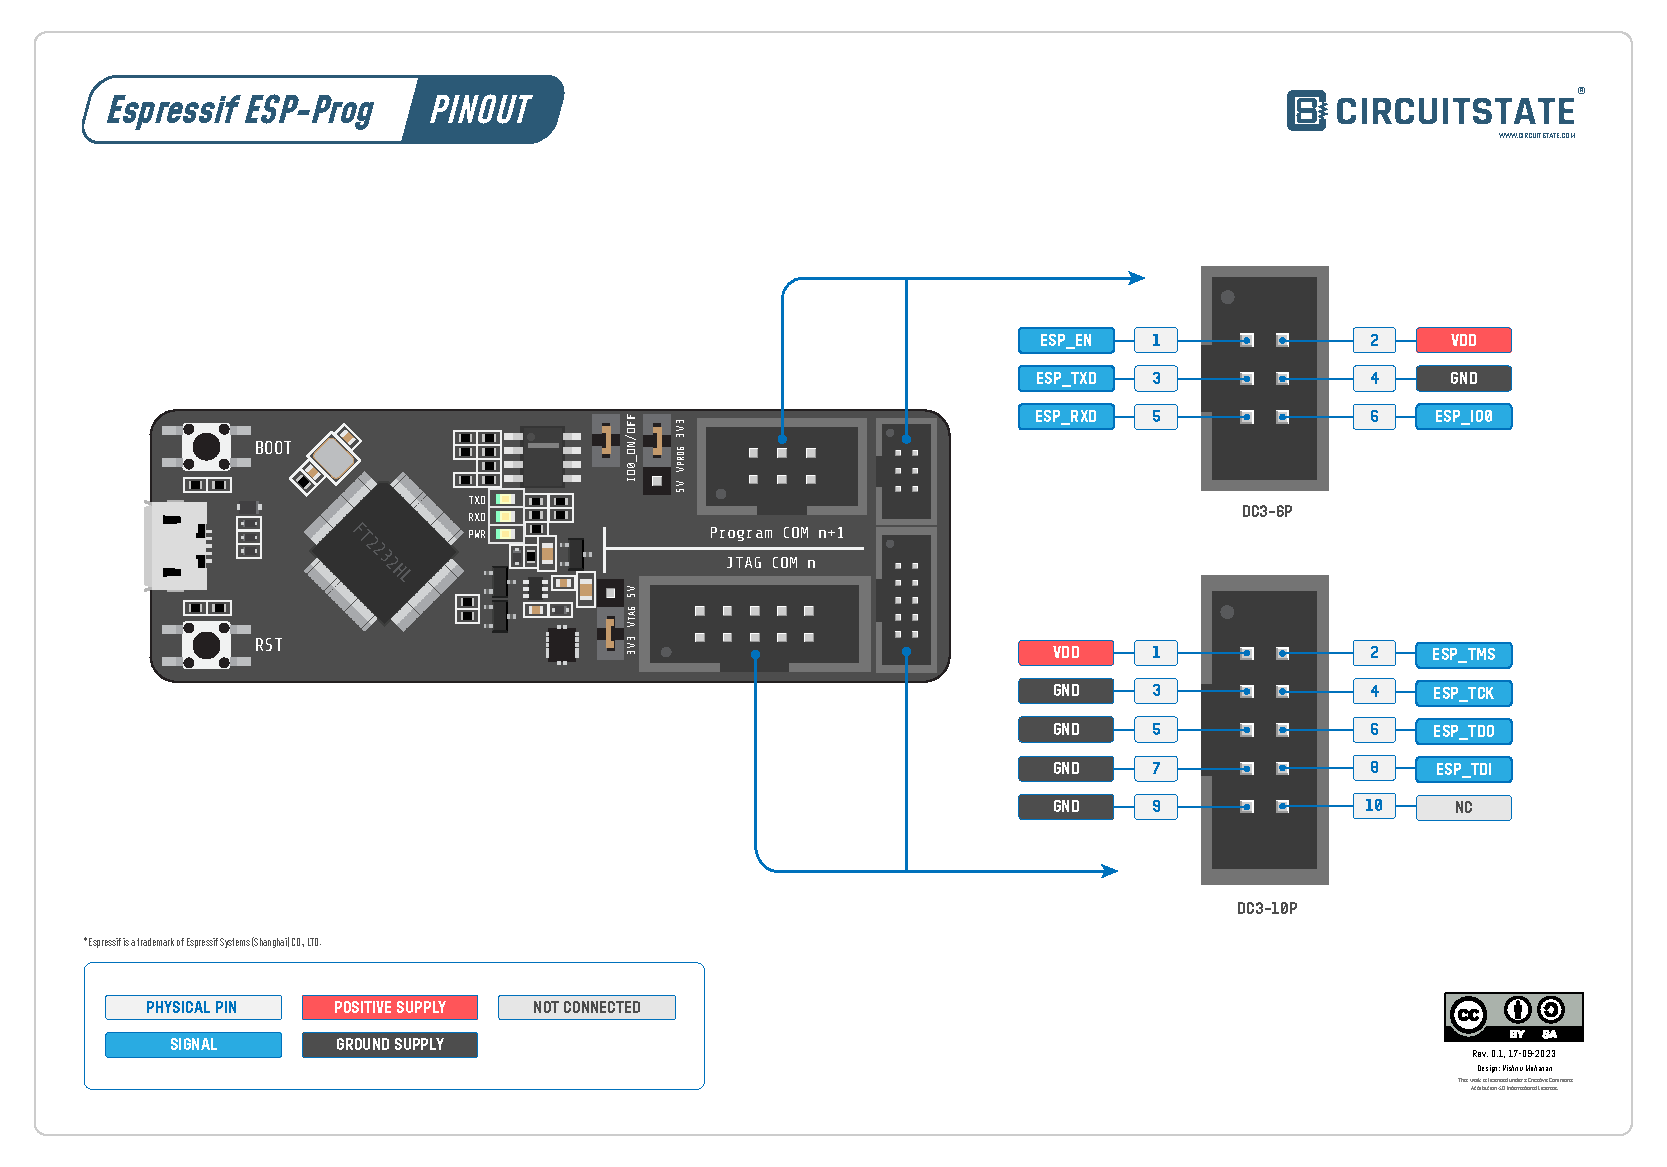
\includegraphics[width=0.8\textwidth]{figures/esp-prog-pinout.pdf}
    \caption{Diagrama del dispositivo ESP-Prog~\cite{esp-prog-pinout}.}
    \label{fig:esp-prog-pinout}
\end{figure}

Para poder utilizarlo correctamente, se deberá llevar a cabo la siguiente conexión~\cite{esp-prog-conn}:

\begin{itemize}
    \item Pin 1 ($V_{DD}$) de DC3-10P de ESP-Prog a pin 3V3 del dispositivo ESP32.
    \item Pin 2 (ESP\_TMS) de DC3-10P de ESP-Prog al pin 14 del dispositivo ESP32.
    \item Pin 3 (GND) de DC3-10P de ESP-Prog a pin GND del dispositivo ESP32.
    \item Pin 4 (ESP\_TCK) de DC3-10P de ESP-Prog al pin 13 del dispositivo ESP32.
    \item Pin 6 (ESP\_TD0) de DC3-10P de ESP-Prog al pin 15 del dispositivo ESP32.
    \item Pin 8 (ESP\_TD1) de DC3-10P de ESP-Prog al pin 12 del dispositivo ESP32.
    \item Pin 1 (ESP\_EN) de DC3-6P de ESP-Prog a pin EN del dispositivo ESP32.
    \item Pin 3 (ESP\_TXD) de DC3-6P de ESP-Prog a pin TX del dispositivo ESP32.
    \item Pin 5 (ESP\_RXD) de DC3-6P de ESP-Prog a pin RX del dispositivo ESP32.
    \item Pin 6 (ESP\_IO0) de DC3-6P de ESP-Prog al pin 0 del dispositivo ESP32.
\end{itemize}

A la hora de carga el \textit{software}, se deberá hacer mediante una conexión JTAG.
Sin embargo, si no se utilizase el dispositivo ESP-Prog, se debería emplear una conexión \ac{UART}.


\subsection{Dilithium}\label{subsec:dilithium}

En primer lugar, se debe obtener el código de referencia de este algoritmo sobre el cual trabajar a continuación.
Este código se ha obtenido desde el repositorio oficial de CRYSTALS-Dilithium~\cite{github-dilithium}.
Dentro de este repositorio, se ha utilizado la implementación de referencia \texttt{ref}, ya que la restante, \texttt{avx2}, se encuentra optimizada para procesadores Intel con arquitectura x86.

Una vez se ha seleccionado el código a utilizar, se debe crear un proyecto que lo incluya.
Para ello, se ha creado un nuevo proyecto utilizando la extensión de Espressif en VSCode.
Los ficheros de este repositorio se han organizado tal y como se puede apreciar en la Figura~\ref{tree:dilithium}.

\begin{figure}[H]
\centering
\framebox[\textwidth]{%
\begin{minipage}{10cm}
\dirtree{%
.1 Dilithium.
.2 CMakeLists.txt.
.2 main.
.3 CMakeLists.txt.
.3 main.c.
.3 src.
.4 aes256ctr.c.
.4 fips202.c.
.4 ntt.c.
.4 packing.c.
.4 poly.c.
.4 polyvec.c.
.4 randombytes.c.
.4 reduce.c.
.4 rounding.c.
.4 sign.c.
.4 symmetric-aes.c.
.4 symmetric-shake.c.
.3 include.
.4 aes256ctr.h.
.4 api.h.
.4 config.h.
.4 fips202.h.
.4 main.h.
.4 ntt.h.
.4 packing.h.
.4 params.h.
.4 poly.h.
.4 polyvec.h.
.4 randombytes.h.
.4 reduce.h.
.4 rounding.h.
.4 sign.h.
.4 symmetric.h.
}
\end{minipage}
}
\caption{Árbol de ficheros del proyecto Dilithium.}
\label{tree:dilithium}
\end{figure}

\subsubsection{Ficheros CMake}\label{subsubsec:dilithium-cmake}

En este árbol, el archivo con ruta \texttt{Dilithium/CMakeLists.txt} únicamente especifica la versión mínima del módulo CMake para evitar posibles incompatibilidades, la inclusión del archivo \texttt{project.cmake} y la definición del nombre del proyecto.
Todo esto se refleja en el Código~\ref{lst:dilithium-cmake}.
El contenido de este fichero se ha creado teniendo en cuenta los ficheros análogos del resto de proyectos que da ESP-IDF como ejemplo.

\begin{lstlisting}[label={lst:dilithium-cmake},style=Bashnice,firstnumber=1,caption={Archivo \texttt{Dilithium/CMakeLists.txt}.}]
cmake_minimum_required(VERSION 3.16)

include($ENV{IDF_PATH}/tools/cmake/project.cmake)
project(Dilithium)
\end{lstlisting}

Dentro del directorio \texttt{main}, se han creado dos subdirectorios: \texttt{src} y \texttt{include}.
En el primero de ellos, se incluyen todos los archivos de código fuente de los que hace uso el algoritmo mientras que en el segundo de ellos se incluyen todas las librerías necesarias para su correcto funcionamiento.

Es necesario incluir, dentro del diretorio \texttt{main}, otro archivo \texttt{CMakeLists.txt} en el cual se especifiquen los archivos a incluir en la compilación del \textit{software}.
Por ello, se han incluido todos los archivos del directorio \texttt{src} como archivos fuente y el directorio \texttt{include} como directorio de librerías, tal y como se muestra en el Código~\ref{lst:dilithium-main-cmake}.

\begin{lstlisting}[label={lst:dilithium-main-cmake},style=Bashnice,firstnumber=1,caption={Archivo \texttt{Dilithium/main/CMakeLists.txt}.}]
idf_component_register(SRCS "main.c" "./src/sign.c" "./src/packing.c" "./src/polyvec.c" "./src/poly.c" "./src/ntt.c" "./src/reduce.c" "./src/rounding.c" "./src/symmetric-shake.c" "./src/symmetric-aes.c" "./src/fips202.c" "./src/aes256ctr.c" "./src/randombytes.c"
                    INCLUDE_DIRS "include")
\end{lstlisting}

\subsubsection{Generación de números aleatorios}\label{subsubsec:dilithium-random}

Un aspecto esencial consiste en la generación de número aleatorios.
Para ello, se dispone del archivo \texttt{Dilithium/main/src/randombytes.c}.
En él, se incluye la definición de la función \texttt{randombytes} (utilizada para la generación de números aleatorios de una determinada longitud) tanto para un dispositivo utilizando el sistema operativo Windows o uno basado en Linux, como se puede apreciar en el Código~\ref{lst:dilithium-randombytes}.
Inicialmente, se incluye la versión del sistema Linux ya que la compilación se lleva a cabo en un dispositivo con el sistema operativo Ubuntu 220.4 LTS.

\begin{lstlisting}[label={lst:dilithium-randombytes},style=Cnice,firstnumber=1,caption={Archivo \texttt{Dilithium/main/src/randombytes.c}.}]
#ifdef _WIN32
void randombytes(uint8_t *out, size_t outlen) {
  HCRYPTPROV ctx;
  size_t len;

  if(!CryptAcquireContext(&ctx, NULL, NULL, PROV_RSA_FULL, CRYPT_VERIFYCONTEXT))
    abort();

  while(outlen > 0) {
    len = (outlen > 1048576) ? 1048576 : outlen;
    if(!CryptGenRandom(ctx, len, (BYTE *)out))
      abort();

    out += len;
    outlen -= len;
  }

  if(!CryptReleaseContext(ctx, 0))
    abort();
}
#elif defined(__linux__) && defined(SYS_getrandom)
void randombytes(uint8_t *out, size_t outlen) {
  ssize_t ret;

  while(outlen > 0) {
    ret = syscall(SYS_getrandom, out, outlen, 0);
    if(ret == -1 && errno == EINTR)
      continue;
    else if(ret == -1)
      abort();

    out += ret;
    outlen -= ret;
  }
}
\end{lstlisting}

Teniendo esto en cuenta, es necesaria la inclusión de una opción indicada para el dispositivo ESP32 y la compilación de esta en vez de la diseñada para los sistemas basados en Linux.
Para ello, se ha añadido la definición especificada en el Código~\ref{lst:dilithium-randombytes-esp32}.
En ella, se utiliza la función \texttt{esp\_fill\_random}~\cite{esp32-random} la cual genera un número aleatorio de longitud \texttt{outlen} y lo almacena en \texttt{out}.
Estos números aleatorios son generados mediante una fuente \textit{hardware}.

\begin{lstlisting}[label={lst:dilithium-randombytes-esp32},style=Cnice,firstnumber=1,caption={Generación de números aleatorios para ESP32.}]
#elif defined(ESP32)
#include "esp_random.h"

void randombytes(uint8_t *out, size_t outlen) {
  esp_fill_random(out, outlen);
}
#endif
\end{lstlisting}


\subsubsection{Fichero de comprobación}\label{subsubsec:dilithium-main}

Una vez se han incluido y referenciado todos los archivos, es necesario crear una prueba que nos permita comprobar la ejecución del algoritmo.
Para ello, se ha creado el archivo \texttt{main.c}, el cual está formado por el contenido mostrado en el Código~\ref{lst:dilithium-main}.
En este fichero, se ejecuta la generación de claves (\texttt{crypto\_sign\_keypair}) y se comprueba si ha existido algún error en la generación.
Una vez se han obtenido las claves pública (\texttt{pk}) y privada (\texttt{sk}), se lleva a cabo la firma de un mensaje previamente especificado (\texttt{m} con longitud \texttt{mlen}) con la función \texttt{crypto\_sign}.
El resultado de esta operación se almacena en la variable \texttt{sm} con longitud \texttt{smlen} y se comprueba si esta firma se ha relizado correctamente.
Finalmente, se lleva a cabo la función de comprobación de firma con la función \texttt{crypto\_sign\_open}.
Una vez realizada, se almacena el mensaje recuperado en la variable \texttt{m1} con longitud \texttt{mlen1}.
Para comprobar la integridad de este mensaje, se compara la longitud y contenido del mensaje recuperado y del mensaje inicial.
Si estos dos parámetros coinciden, la prueba ha sido exitosa.

\begin{lstlisting}[label={lst:dilithium-main},style=Cnice,firstnumber=1,caption={Archivo \texttt{Dilithium/main/main.c}.}]
#include <stdio.h>
#include <string.h>

#include "api.h"
#include "main.h"
    
void app_main(void)
{
    printf("Inicio con la opción %d\n\r", DILITHIUM_MODE);

    //Generación de claves
    uint8_t *pk = (uint8_t*) malloc(CRYPTO_PUBLICKEYBYTES * sizeof(uint8_t));
    uint8_t *sk = (uint8_t*) malloc(CRYPTO_SECRETKEYBYTES * sizeof(uint8_t));
    if (crypto_sign_keypair(pk, sk) != 0) {
        printf("Generacion de claves fallida\n\r");
    } else {
        printf("Generacion de claves exitosa (%d bytes de clave publica y %d bytes de clave privada)\n\r", CRYPTO_PUBLICKEYBYTES, CRYPTO_SECRETKEYBYTES);
    }

    //Firma de mensaje
    uint8_t m[] = "Esto es una prueba de la firma de mensajes utilizando Dilithium.";
    size_t mlen = sizeof(m), smlen;
    uint8_t *sm = (uint8_t *)calloc(mlen+CRYPTO_BYTES, sizeof(uint8_t));
    if (crypto_sign(sm, &smlen, m, mlen, sk) != 0) {
        printf("Firma de mensaje fallida\n\r");
    } else {
        printf("Firma del mensaje exitosa (%d bytes de firma)\n\r", mlen+CRYPTO_BYTES);
    }

    //Comprobación de la firma
    size_t mlen1;
    uint8_t *m1 = (uint8_t *)calloc(mlen+CRYPTO_BYTES, sizeof(uint8_t));
    if (crypto_sign_open(m1, &mlen1, sm, smlen, pk) != 0) {
        printf("Comprobacion de la firma fallida\n\r");
    } else {
        if (mlen != mlen1) {
            printf("Longitud del mensaje original distinta a la longitud del mensaje recuperado\n\r");
        } else if (memcmp(m, m1, mlen)) {
            printf("Contenido del mensaje original distinto al contenido del mensaje recuperado\n\r");
        } else {
            printf("Comprobacion de la firma del mensaje exitosa (%d bytes de mensaje)\n\r", mlen1);
        }
    }

    //Liberación de la memoria reservada
    free(pk);
    free(sk);
    free(m1);
    free(sm);
}
\end{lstlisting}

Como se puede observar en el Código~\ref{lst:dilithium-main}, se hace referencia al fichero \texttt{main.h}.
Este fichero únicamente contiene la especificación de la versión del algoritmo mediante la definición de \texttt{DILITHIUM\_MODE}, como se muestra en el Código~\ref{lst:dilithium-mainh}.
También, se elimina la definición previa de \texttt{\_\_linux\_\_} y la definición de \texttt{ESP32}, cuyo motivo se trata en la apartado~\ref{subsubsec:dilithium-random}.

\begin{lstlisting}[label={lst:dilithium-mainh},style=Cnice,firstnumber=1,caption={Archivo \texttt{Dilithium/main/include/main.h}.}]
#ifndef MAIN_H
#define MAIN_H

//Necesario para generación de números aleatorios
#ifdef __linux__
    #undef __linux__
#endif
#ifndef ESP32
    #define ESP32
#endif

#ifndef DILITHIUM_MODE
    #define DILITHIUM_MODE 3	/*{2,3,5}*/
#endif
#endif
\end{lstlisting}


\subsubsection{Uso de memoria dinámica}\label{subsubsec:dilithium-dynamic}

Una vez realizados todos los pasos anteriores, el siguiente paso consiste en la ejecución de la comprobación del algoritmo.
Al ejecutarlo, se comprueba que la ejecución se bloquea en la generación de claves sin mostrar ningún código de error.
LLevando a cabo distinta comprobaciones, se encontró que le error sucedía en la función \texttt{KeccakF1600\_StatePermute} dentro del archivo \texttt{fips202.c}, aunque no se puedo concretar la instrucción exacta en la que sucedía el error.
Por ello, se ha requerido utilizar el depurador ESP-Prog.
A través del depurador, se ha concluido que el error surge del error que se aprecia en la Captura~\ref{}.

%//TODO: captura error depurador

Según se ha encontrado en distintas entradas del foro oficial de ESP32~\cite{esp32-forum1}~\cite{esp32-forum2}~\cite{esp32-forum2}, este error se debe, sin duda, a un problema en la memoria del dispositivo.
En una de estas entradas, se sugiere la posibilidad de un \textit{overflow} del \textit{stack} sea el causante de este problema.
Este problema surge del hecho de que, antes de ejecutar el programa de prueba, se realiza una reserva de memoria automáticamente y la cantidad de memoria reservada es inferior a la necesitada posteriormente.
Por ello, se debe hacer uso de la memoria \textit{heap} en vez de la memoria \textit{stack}.
Con esta idea en mente, se ha llevado a cabo la modificación de la implementación inicial para hacer uso de memoria dinámica y evitar el \textit{overflow} del \textit{stack} al requerir un tamaño mucho menor de esta memoria.
De esta forma, la cantidad de memoria reservada inicialmente no será sobrepasada por la cantidad de memoria en \textit{stack} requerida.

Las primeras variables en ser modificadas han sido las incluidas en el archivo \texttt{main.c}, las cuales representan las claves pública, privada y firma del mensaje y, por ende, una gran cantidad de datos (1312, 2528 y 2420 bytes respectivamente en Dilithium2).
Esto se puede apreciar en el Código~\ref{lst:dilithium-main}.

\begin{lstlisting}[label={lst:dilithium-key-dyn},style=Cnice,firstnumber=1,caption={Modificación de la función \texttt{crypto\_sign\_keypair} en el archivo \texttt{Dilithium/main/src/sign.c}.}]
int crypto_sign_keypair(uint8_t *pk, uint8_t *sk) {
  uint8_t seedbuf[2*SEEDBYTES + CRHBYTES];
  uint8_t tr[SEEDBYTES];
  const uint8_t *rho, *rhoprime, *key;
  polyvecl *mat = (polyvecl*) malloc(K * sizeof(polyvecl));
  polyvecl *s1 = (polyvecl*) malloc( sizeof(polyvecl));
  polyvecl *s1hat = (polyvecl*) malloc( sizeof(polyvecl));
  polyveck *s2 = (polyveck*) malloc( sizeof(polyveck));
  polyveck *t1 = (polyveck*) malloc( sizeof(polyveck));
  polyveck *t0 = (polyveck*) malloc( sizeof(polyveck));

  ...

  free(mat);
  free(s1);
  free(s1hat);
  free(s2);
  free(t1);
  free(t0);

  return 0;
}
\end{lstlisting}

En la modificación mostrada en el Código~\ref{lst:dilithium-key-dyn}, se han priorizado las variables de mayor tamaño, como en este caso todas las variables del tipo \texttt{polyvecl}, ya que esta estructura consta de un tamaño de 4 kB en Dilithium2, 6 kB en Dilithium3 y 8 kB en Dilithium5.
También, las variables de tipo \texttt{polyveck} ya que esta estructura requiere de un tamaño de 4 kB en Dilithium2, 5 kB en Dilithium3 y 7 kB en Dilithium5.

\begin{lstlisting}[label={lst:dilithium-sign-dyn},style=Cnice,firstnumber=1,caption={Modificación de la función \texttt{crypto\_sign\_signature} en el archivo \texttt{Dilithium/main/src/sign.c}.}]
int crypto_sign_signature(uint8_t *sig, size_t *siglen, const uint8_t *m, size_t mlen, const uint8_t *sk)
{
  unsigned int n;
  uint8_t seedbuf[3*SEEDBYTES + 2*CRHBYTES];
  uint8_t *rho, *tr, *key, *mu, *rhoprime;
  uint16_t nonce = 0;
  polyvecl *mat = (polyvecl*) malloc(K * sizeof(polyvecl));
  polyvecl *s1 = (polyvecl*) malloc(sizeof(polyvecl));
  polyvecl *y  = (polyvecl*) malloc(sizeof(polyvecl));
  polyvecl *z  = (polyvecl*) malloc(sizeof(polyvecl));

  polyveck *t0 = (polyveck*) malloc(sizeof(polyveck));
  polyveck *s2 = (polyveck*) malloc(sizeof(polyveck));
  polyveck *w1 = (polyveck*) malloc(sizeof(polyveck));
  polyveck *w0 = (polyveck*) malloc(sizeof(polyveck));
  polyveck *h  = (polyveck*) malloc(sizeof(polyveck));
  poly *cp = (poly*) malloc(sizeof(poly));
  keccak_state *state = (keccak_state*) malloc(sizeof(keccak_state));

  ...

  free(mat);
  free(s1);
  free(y);
  free(z);
  free(t0);
  free(s2);
  free(w1);
  free(w0);
  free(h);
  free(cp);
  free(state);

  return 0;
}
\end{lstlisting}

A continuación, se modificó la función \texttt{crypto\_sign\_signature} mediante el Código~\ref{lst:dilithium-sign-dyn}.
En este caso, se han alterado las variables de tipo \texttt{polyveck} y \texttt{polyvecl} por el mismo motivo explicado anteriormente.
Además, se han adaptado las variables \texttt{cp} y \texttt{state} a pesar de no requerir una gran cantidad de memoria.

\begin{lstlisting}[label={lst:dilithium-ver-dyn},style=Cnice,firstnumber=1,caption={Modificación de la función \texttt{crypto\_sign\_verify} en el archivo \texttt{Dilithium/main/src/sign.c}.}]
int crypto_sign_verify(const uint8_t *sig,
                       size_t siglen,
                       const uint8_t *m,
                       size_t mlen,
                       const uint8_t *pk)
{
  unsigned int i;
  uint8_t *buf = (uint8_t *)malloc((K*POLYW1_PACKEDBYTES) * sizeof(uint8_t));
  uint8_t rho[SEEDBYTES];
  uint8_t mu[CRHBYTES];
  uint8_t c[SEEDBYTES];
  uint8_t c2[SEEDBYTES];
  poly *cp = (poly*) malloc(sizeof(poly));
  polyvecl *mat = (polyvecl*) malloc(K * sizeof(polyvecl));
  polyvecl *z   = (polyvecl*) malloc(sizeof(polyvecl));;

  polyveck *t1 = (polyveck*) malloc(sizeof(polyveck));
  polyveck *w1 = (polyveck*) malloc(sizeof(polyveck));
  polyveck *h = (polyveck*) malloc(sizeof(polyveck));
  keccak_state *state = (keccak_state*) malloc(sizeof(keccak_state));

  ...

  free(buf);
  free(cp);
  free(mat);
  free(z);
  free(t1);
  free(w1);
  free(h);
  free(state);

  return 0;
}
\end{lstlisting}

Por último, se ha modificado la función \texttt{crypto\_sign\_verify} tal y como se muestra en el Código~\ref{lst:dilithium-ver-dyn}.
Para esta modificación se ha seguido la pauta anteriormente especificada, en la cual se modifican las variables de tipo \texttt{polyveck} \texttt{polyvecl}.
Además, en este caso, se ha modificado la variable \texttt{buf} ya que esta necesitaría 768 bytes en Dilithium2 y Dilithium3 y 1 kB en el caso de Dilithium5.

Una vez realizadas todas estas modificaciones, se han adaptado las llamadas a las funciones que componen \texttt{crypto\_sign\_keypair}, \texttt{crypto\_sign\_signature} y \texttt{crypto\_sign\_verify} de forma que se utilicen correctamente los punteros creados en lugar de las variables utilizadas anteriormente.


\subsubsection{Comprobación del algoritmo}\label{subsubsec:dilithium-compro}

Tras completar todos los pasos indicados previamente, se lleva a cabo la ejecución del algoritmo.
Esta ejecución se lleva a cabo mediante el programa mostrado en el Código~\ref{lst:dilithium-main}.
El resultado de esta ejecución se muestra en la Captura~\ref{fig:dilithium-check}.

\begin{figure}[h]
    \centering
    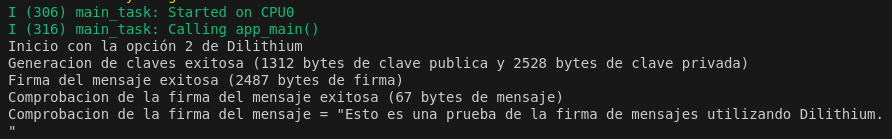
\includegraphics[width=0.5\textwidth]{figures/dilithium-check.png}
    \caption{Comprobación de ejecución de algoritmo Dilithium.}
    \label{fig:dilithium-check}
\end{figure}



\subsection{Kyber}\label{subsec:kyber}

\begin{figure}[H]
\centering
\framebox[\textwidth]{%
\begin{minipage}{10cm}
\dirtree{%
.1 Kyber.
.2 CMakeLists.txt.
.2 main.
.3 CMakeLists.txt.
.3 main.c.
.3 src.
.4 aes256ctr.c.
.4 cbd.c.
.4 cpucycles.c.
.4 fips202.c.
.4 indcpa.c.
.4 kem.c.
.4 kex.c.
.4 ntt.c.
.4 poly.c.
.4 polyvec.c.
.4 randombytes.c.
.4 reduce.c.
.4 rng.c.
.4 sha256.c.
.4 sha512.c.
.4 speed\_print.c.
.4 symmetric-aes.c.
.4 symmetric-shake.c.
.4 verify.c.
.3 include.
.4 aes256ctr.h.
.4 api.h.
.4 cbd.h.
.4 cpucycles.h.
.4 fips202.h.
.4 indcpa.h.
.4 kem.h.
.4 kex.h.
.4 main.h.
.4 ntt.h.
.4 params.h.
.4 poly.h.
.4 polyvec.h.
.4 randombytes.h.
.4 reduce.h.
.4 rng.h.
.4 sha2.h.
.4 speed\_print.h.
.4 symmetric.h.
.4 verify.h.
}
\end{minipage}
}
\caption{Árbol de ficheros del proyecto Kyber.}
\label{tree:kyber}
\end{figure}

Al igual que para el caso de Dilithium~\ref{subsec:dilithium}, el primer paso consiste en seleccionar la implementación a tratar.
Para ello, se ha utilizado el repositorio oficial de CRYSTALS-Kyber~\cite{github-kyber}.
Dentro de este código, existe tanto una implementación estándar dentro del directorio \texttt{ref} y otra optimizada para procesadores Intel x86 bajo el nombre \texttt{avx2}.

Repitiendo los pasos descritos para Dilithium, se ha procedido a crear un proyecto mediante la extensión de Espressif en VSCode.
El árbol de ficheros utilizado es el mostrado en la Figura~\ref{tree:kyber}.

\subsubsection{Ficheros CMake}\label{subsubsec:kyber-cmake}

Dentro de este árbol, el archivo \texttt{Kyber/CMakeLists.txt} indica la versión mínima aceptada del módulo CMake para evitar posibles incompatibilidades, el uso del archivo \texttt{project.cmake} y el nombre del proyecto.
Todo esto se refleja en el Código~\ref{lst:kyber-cmake}.
El contenido de este fichero se ha creado teniendo en cuenta los ficheros análogos del resto de proyectos que da ESP-IDF como ejemplo.

\begin{lstlisting}[label={lst:kyber-cmake},style=Bashnice,firstnumber=1,caption={Archivo \texttt{Kyber/CMakeLists.txt}.}]
cmake_minimum_required(VERSION 3.16)

include($ENV{IDF_PATH}/tools/cmake/project.cmake)
project(Kyber)
\end{lstlisting}

Dentro del directorio \texttt{main}, se han creado dos subdirectorios: \texttt{src} y \texttt{include}.
En el primero de ellos, se incluyen todos los archivos de código fuente de los que hace uso el algoritmo mientras que en el segundo de ellos se incluyen todas las librerías necesarias para su correcto funcionamiento.

Es necesario incluir, dentro del diretorio \texttt{main}, otro archivo \texttt{CMakeLists.txt} en el cual se especifiquen los archivos a incluir en la compilación del \textit{software}.
Por ello, se han incluido todos los archivos del directorio \texttt{src} como archivos fuente y el directorio \texttt{include} como directorio de librerías, tal y como se muestra en el Código~\ref{lst:kyber-main-cmake}.

\begin{lstlisting}[label={lst:kyber-main-cmake},style=Bashnice,firstnumber=1,caption={Archivo \texttt{Kyber/main/CMakeLists.txt}.}]
idf_component_register(SRCS "main.c" "src/kex.c" "src/kem.c" "src/indcpa.c" "src/polyvec.c" "src/poly.c" "src/cbd.c" "src/ntt.c" "src/reduce.c" "src/verify.c" "src/symmetric-shake.c" "src/symmetric-aes.c" "src/fips202.c" "src/randombytes.c"
    INCLUDE_DIRS "include")
\end{lstlisting}

\subsubsection{Generación de números aleatorios}\label{subsubsec:kyber-random}

Teniendo en cuenta que el dispositivo utilizado es el mismo que para el algoritmo Dilithium, la generación de números aleatorios se realiza de la misma manera que la mostrada en el Código~\ref{lst:dilithium-randombytes-esp32}.
Además, debido a que tanto Dilithium como Kyber comparten creadores, la generación de números aleatorios es idéntica, por lo que el archivo de generación de números aleatorios \texttt{Kyber/main/src/randombytes.c} es el mismo y, por ende, la forma en la que incluir la versión para el ESP32.

\subsubsection{Fichero de comprobación}\label{subsubsec:kyber-main}

Una vez se han incluido y referenciado todos los archivos, es necesario crear una prueba que nos permita comprobar la ejecución del algoritmo.
Para ello, se ha creado el archivo \texttt{main.c}, el cual está formado por el contenido mostrado en el Código~\ref{lst:kyber-main}.
En primer lugar, se llama a la función \texttt{crypto\_kem\_keypair}, encargada de generar las claves tanto pública como privada a utilizar.
La clave pública se almacenará en la variable \texttt{pk} mientras que la clave privada estará representada por \texttt{sk}.
Si esta generación fuese errónea, la ejecución finalizaría.
En caso contrario, se llevaría a cabo la generación del secreto compartido (\texttt{ss\_pub}) y del texto cifrado (\texttt{ct}) haciendo uso de la clave pública mediante la función \texttt{crypto\_kem\_enc}.
A continuación, se utiliza la función \texttt{crypto\_kem\_dec}, a la cual se entrega el texto cifrado \texttt{ct} generado por la función anterior y la clave privada y devuelve el secreto compartido \texttt{ss\_priv}, el cual, si la ejecución ha sido correcta, debería coincidir con el secreto generado anteriormente \texttt{ss\_pub}.
Para finalizar, se lleva a cabo esta verificación y se libera la memoria correspondiente a las variables creadas al inicio del programa.

\begin{lstlisting}[label={lst:kyber-main},style=Cnice,firstnumber=1,caption={Archivo \texttt{Kyber/main/main.c}.}]
#include <stdio.h>
#include <stdlib.h>
#include <string.h>
#include <ctype.h>

#include "main.h"
#include "kem.h"
#include "api.h"

#include "randombytes.h"

void app_main (void)
{
    printf("Inicio con la opción %d\n\r", KYBER_K);

    //Generación de claves
    unsigned char *pk = (unsigned char*) malloc(CRYPTO_PUBLICKEYBYTES * sizeof(unsigned char));
    unsigned char *sk = (unsigned char*) malloc(CRYPTO_SECRETKEYBYTES * sizeof(unsigned char));
    if (crypto_kem_keypair(pk, sk) != 0) {
        printf("Generacion de claves fallida\n\r");
        return;
    } else {
        printf("Generacion de claves exitosa (%d bytes de clave publica y %d bytes de clave privada)\n\r", CRYPTO_PUBLICKEYBYTES, CRYPTO_SECRETKEYBYTES);
    }

    //Generación de texto cifrado y secreto compartido
    unsigned char *ct = (unsigned char*) malloc(CRYPTO_CIPHERTEXTBYTES * sizeof(unsigned char));
    unsigned char *ss_pub = (unsigned char*) malloc(CRYPTO_BYTES * sizeof(unsigned char));
    if (crypto_kem_enc(ct, ss_pub, pk) != 0) {
        printf("Generacion de texto cifrado y secreto compartido fallida\n\r");
        return;
    } else {
        printf("Generacion de texto cifrado y secreto compartido exitosa (%d bytes de texto cifrado y %d bytes de secreto compartido)\n\r", CRYPTO_CIPHERTEXTBYTES, CRYPTO_BYTES);
    }

    //Generación de secreto compartido
    unsigned char *ss_priv = (unsigned char*) malloc(CRYPTO_BYTES * sizeof(unsigned char));
    if (crypto_kem_dec(ss_priv, ct, sk) != 0) {
        printf("Generacion de secreto compartido fallida\n\r");
        return;
    } else {
        printf("Generacion de secreto compartido exitosa (%d bytes de secreto compartido)\n\r", CRYPTO_BYTES);
    }

    //Comprobación de resultados
    if (memcmp(ss_pub, ss_priv, (unsigned int) CRYPTO_BYTES) ) {
        printf("Comprobación fallida\n\r");
    } else{
        printf("¡Comprobación superada!\n\r");
    }

    //Liberación de la memoria reservada
    free(pk);
    free(sk);
    free(ct);
    free(ss_pub);
    free(ss_priv);
}
\end{lstlisting}

Como se puede observar en el Código~\ref{lst:kyber-main}, se hace referencia al fichero \texttt{main.h}.
Este fichero únicamente contiene la especificación de la versión del algoritmo mediante la definición de \texttt{KYBER\_K}, como se muestra en el Código~\ref{lst:kyber-mainh}.
En este código, si \texttt{KYBER\_K} se hace uso de Kyber512, si vale 3 se utiliza Kyber768 y, si vale 4, se emplea Kyber1024.
También, se elimina la definición previa de \texttt{\_\_linux\_\_} y la definición de \texttt{ESP32}, cuyo motivo se trata en la apartado~\ref{subsubsec:dilithium-random}.

\begin{lstlisting}[label={lst:kyber-mainh},style=Cnice,firstnumber=1,caption={Archivo \texttt{Kyber/main/include/main.h}.}]
#ifndef MAIN_H
#define MAIN_H

//Necesario para generación de números aleatorios
#ifdef __linux__
    #undef __linux__
#endif
#ifndef ESP32
    #define ESP32
#endif

#ifndef KYBER_K
    #define KYBER_K 3
#endif
#endif
\end{lstlisting}


\subsubsection{Uso de memoria dinámica}\label{subsubsec:kyber-dynamic}

De la misma manera que Dilithium suponía un \textit{overflow} en el \textit{stack} reservado, Kyber también, como se puede comprobar en la Figura~\ref{}.

%//TODO: captura error depurador

Por ello, se han seguido los mismos pasos y se ha hecho uso de la \textit{heap} cambiando las variables estáticas que más memoria requerían a ser variables dinámicas.
El archivo en ser modificado ha sido el archivo \texttt{Kyber/main/src/indcpa.c}.
En él, se ha cambiado la función \texttt{indcpa\_keypair} tal y como se indica en el Código~\ref{lst:kyber-key-dyn}.

\begin{lstlisting}[label={lst:kyber-key-dyn},style=Cnice,firstnumber=1,caption={Modificación de la función \texttt{indcpa\_keypair} en el archivo \texttt{Kyber/main/src/indcpa.c}.}]
void indcpa_keypair(uint8_t pk[KYBER_INDCPA_PUBLICKEYBYTES], uint8_t sk[KYBER_INDCPA_SECRETKEYBYTES])
{
  unsigned int i;
  uint8_t *buf = (uint8_t*) malloc(2*KYBER_SYMBYTES * sizeof(uint8_t));
  const uint8_t *publicseed = buf;
  const uint8_t *noiseseed = buf+KYBER_SYMBYTES;
  uint8_t nonce = 0;

  polyvec *a = (polyvec*) malloc(KYBER_K * sizeof(polyvec));
  polyvec *e = (polyvec*) malloc(sizeof(polyvec));
  polyvec *pkpv = (polyvec*) malloc(sizeof(polyvec));
  polyvec *skpv = (polyvec*) malloc(sizeof(polyvec));

  ...

  free(buf);
  free(a);
  free(e);
  free(skpv);
  free(pkpv);
}
\end{lstlisting}

En este caso, las variables de tipo \texttt{polyvec} ocupan 1 kB en le caso de Kyber2, 1.5 kB en el caso de Kyber3 y 2 kB en el caso de Kyber4.
La variable \texttt{a} ocupa un total de 2 kB para Kyber2, 3.5 kB para Kyber3 y 8 kB para Kyber4.
Por ello, todas estas variables han sido modificadas para hacer uso de memoria dinámica en vez de memoria estática, siguiendo el próposito indicado en el apartado~\ref{subsubsec:dilithium-dynamic}.

\begin{lstlisting}[label={lst:kyber-enc-dyn},style=Cnice,firstnumber=1,caption={Modificación de la función \texttt{indcpa\_enc} en el archivo \texttt{Kyber/main/src/indcpa.c}.}]
void indcpa_enc(uint8_t c[KYBER_INDCPA_BYTES], const uint8_t m[KYBER_INDCPA_MSGBYTES], const uint8_t pk[KYBER_INDCPA_PUBLICKEYBYTES], const uint8_t coins[KYBER_SYMBYTES])
{
    unsigned int i;
    uint8_t *seed = (uint8_t*) malloc(KYBER_SYMBYTES * sizeof(uint8_t));
    uint8_t nonce = 0;

    polyvec *sp   = (polyvec*) malloc(sizeof(polyvec));
    polyvec *pkpv = (polyvec*) malloc(sizeof(polyvec));
    polyvec *ep   = (polyvec*) malloc(sizeof(polyvec));
    polyvec *at   = (polyvec*) malloc(KYBER_K * sizeof(polyvec));
    polyvec *b    = (polyvec*) malloc(sizeof(polyvec));

    poly *v   = (poly*) malloc(sizeof(poly));
    poly *k   = (poly*) malloc(sizeof(poly));
    poly *epp = (poly*) malloc(sizeof(poly));

    ...

    free(seed);
    free(sp);
    free(pkpv);
    free(ep);
    free(at);
    free(b);
    free(v);
    free(k);
    free(epp);
}
\end{lstlisting}

En el Código~\ref{lst:kyber-enc-dyn} se observa la modificación realizada en la función encargada de generar el secreto compartido y el texto cifrado.
Para ello, se han modificado las variables del tipo \texttt{polyvec} y del tipo \texttt{poly}, aunque estas últimas requieren una cantidad de memoria mucho menor.

\begin{lstlisting}[label={lst:kyber-dec-dyn},style=Cnice,firstnumber=1,caption={Modificación de la función \texttt{indcpa\_dec} en el archivo \texttt{Kyber/main/src/indcpa.c}.}]
void indcpa_dec(uint8_t m[KYBER_INDCPA_MSGBYTES], const uint8_t c[KYBER_INDCPA_BYTES], const uint8_t sk[KYBER_INDCPA_SECRETKEYBYTES])
{
  polyvec *b    = (polyvec*) malloc(sizeof(polyvec));
  polyvec *skpv = (polyvec*) malloc(sizeof(polyvec));

  poly *v  = (poly*) malloc(sizeof(poly));
  poly *mp = (poly*) malloc(sizeof(poly));

  ...

  free(b);
  free(skpv);
  free(v);
  free(mp);
}
\end{lstlisting}

La última función modificada ha sido la encargad de obtener el secreto compartido apartir del texto cifrado y la clave privada, \texttt{indcpa\_dec}.
Siguiendo los cambios realizados con anterioridad, se han modificado las variables del tipo \texttt{polyvec} y \texttt{poly}.

\subsubsection{Comprobación del algoritmo}\label{subsubsec:kyber-compro}

Para finalizar con este algoritmo, se ha llevado a cabo la comprobación de su funcionamiento utilizando el Código~\ref{lst:kyber-main}.
El resultado de esta ejecución se muestra en la Captura~\ref{fig:kyber-check}.

\begin{figure}[h]
    \centering
    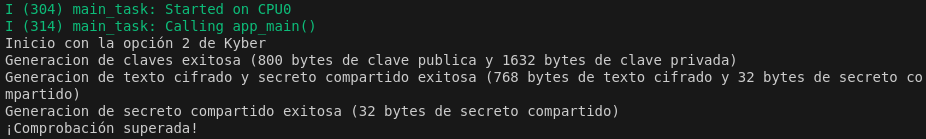
\includegraphics[width=0.5\textwidth]{figures/kyber-check.png}
    \caption{Comprobación de ejecución de algoritmo Kyber.}
    \label{fig:kyber-check}
\end{figure}




\section{RP2040}\label{sec:rp2040}

El siguiente dispositivo a utilizar es el Lyligo T-Display~\cite{lilygo}, el cual incluye un ESP32 y un RP2040.
Este dispositivo utiliza el conector USB-C para programar un elemento u otro, dependiendo si está conectado con una orientación u otra.

Para poder programar el RP2040 se ofrecen varias posibilidades en el repositorio de esta plataforma.
Estas posibilidades son: Arduino, Mycropython y Pico SDK.
Los algoritmos a implementar están desarrollados sobre C, lo cual da un mayor control sobre los recursos del dispositivo.
En cambio, Arduino está implementado en una mezcla de C y C++, por lo que puede no ser óptimo a la hora de utilizar aplicaciones exigentes en lo referente a recursos.
En este aspecto, Micropython tiene el mismo defecto.
Por otro lado, Pico SDK supone directamente una programación en C, lo cual consigue un mejor uso de los recursos disponibles.


\subsection{Pico SDK}\label{subsec:pico-sdk}

La herramienta Pico SDK~\cite{pico-sdk} está desarrollada para otorgar al usuario el mayor control posible sobre el dispositivo.
Este ejecuta un programa con la función \texttt{main} convencional y aporta varias librerías que permiten tratar con temporizadores, conexiones USB y sincronización.

Para la construcción de los projectos, esta herramienta hace uso de CMake ya que es soportado por multitud de IDEs.
Para poder utilizar esta herramienta, se deben seguir los pasos indicados en su repositorio oficial~\cite{pico-sdk-github}.
En primer lugar, se deben instalar los paquetes necesarios con el comando \texttt{sudo apt install cmake gcc-arm-none-eabi libnewlib-arm-none-eabi libstdc++-arm-none-eabi-newlib}.
A continuación, se debe clonar el repositorio de la herramienta con el comando \texttt{git clone https://github.com/raspberrypi/pico-sdk.git}.
Posteriormente, es necesario copiar el archivo \texttt{pico\_sdk\_import.cmake} en el proyecto y establecer la variable de entorno \texttt{PICO\_SDK\_PATH} con la ruta al repositorio recién clonado.
El siguiente paso consiste en crear un archivo CMakeLists.txt como el ejemplo mostrado en el Código~\ref{lst:sdk-example} y el programa que se vaya a ejecutar en el dispositivo.
Por último, se debe crear un directorio \texttt{build} mediante el comando \texttt{mkdir build \&\& cd build \&\& cmake ..} y, dentro del directorio \texttt{build}, ejecutar el comando \texttt{make hello\_world} para construir el ejecutable del programa creado.
Esto genera un archivo .elf para cargar a través de un depurador y un archivo .elf2 para cargar directamente mediante la conexión \ac{USB}.

\begin{lstlisting}[label={lst:sdk-example},style=Cnice,firstnumber=1,caption={Ejemplo de CMakeLists.txt~\cite{pico-sdk-github}.}]
cmake_minimum_required(VERSION 3.13)

# initialize the SDK based on PICO_SDK_PATH
# note: this must happen before project()
include(pico_sdk_import.cmake)

project(my_project)

# initialize the Raspberry Pi Pico SDK
pico_sdk_init()

# rest of your project
\end{lstlisting}


\subsection{HQC-128}\label{subsec:hqc}

El primer algoritmo a implementar en este dispositivo ha sido el algoritmo HQC-128.
Para comenzar, se debe obtener una implementación del mismo.
La implementación seleccionada ha sido la correspondiente al proyecto PQClean~\cite{SSR:KSSW22}.
El código correspondiente a este algoritmo se puede encontrar en su repositorio de GitHub~\cite{pqclean-github}.

Una vez extraídos los archivos correspondientes a este algoritmo, se han colocado de la forma indicada en el árbol de ficheros~\ref{tree:hqc}.

\begin{figure}[H]
\centering
\framebox[\textwidth]{%
\begin{minipage}{10cm}
\dirtree{%
.1 HQC-128.
.2 main.c.
.2 CMakeLists.txt.
.2 src.
.3 code.c.
.3 fft.c.
.3 fips202.c.
.3 gf.c.
.3 gf2x.c.
.3 hqc.c.
.3 kem.c.
.3 parsing.c.
.3 randombytes.c.
.3 reed\_muller.c.
.3 reed\_solomon.c.
.3 shake\_ds.c.
.3 shake\_prng.c.
.3 vector.c.
.2 include.
.3 api.h.
.3 code.h.
.3 fft.h.
.3 fips202.h.
.3 gf.h.
.3 gf2x.h.
.3 hqc.h.
.3 main.h.
.3 parameters.h.
.3 parsing.h.
.3 randombytes.h.
.3 reed\_muller.h.
.3 reed\_solomon.h.
.3 shake\_ds.h.
.3 shake\_prng.h.
.3 vector.h.
}
\end{minipage}
}
\caption{Árbol de ficheros del proyecto HQC-128.}
\label{tree:hqc}
\end{figure}

Este proyecto incluye, al igual que los proyectos del dispositivo ESP32, todos los ficheros de código fuente en un directorio \texttt{src} y todas librerías en un directorio \texttt{include}.
Además, dispone de un archivo CMakeLists.txt que se explica en el apartado~\ref{subsubsec:hqc-cmake} y un archivo de comprobación que se detalla en el apartado~\ref{subsubsec:hqc-main}.


\subsubsection{Fichero CMake}\label{subsubsec:hqc-cmake}

Dentro de este archivo CMakelists.txt, se puede hallar el contenido del Código~\ref{lst:hqc-make}.

\begin{lstlisting}[label={lst:hqc-make},style=Cnice,firstnumber=1,caption={Archivo \texttt{HQC-128/CMakeLists.txt}.}]
cmake_minimum_required(VERSION 3.13)

if (TARGET tinyusb_device)
    add_compile_options(-Wall -Wextra -Wpedantic -Wredundant-decls -Wcast-align -Wmissing-prototypes -DPQCLEAN_NAMESPACE=PQCLEAN_HQC128_CLEAN)

    add_executable(hqc-128)

    target_sources(hqc-128 PUBLIC
            ${CMAKE_CURRENT_LIST_DIR}/main.c
            ${CMAKE_CURRENT_LIST_DIR}/src/code.c
            ${CMAKE_CURRENT_LIST_DIR}/src/fft.c
            ${CMAKE_CURRENT_LIST_DIR}/src/gf.c
            ${CMAKE_CURRENT_LIST_DIR}/src/gf2x.c
            ${CMAKE_CURRENT_LIST_DIR}/src/hqc.c
            ${CMAKE_CURRENT_LIST_DIR}/src/kem.c
            ${CMAKE_CURRENT_LIST_DIR}/src/parsing.c
            ${CMAKE_CURRENT_LIST_DIR}/src/reed_muller.c
            ${CMAKE_CURRENT_LIST_DIR}/src/reed_solomon.c
            ${CMAKE_CURRENT_LIST_DIR}/src/shake_ds.c
            ${CMAKE_CURRENT_LIST_DIR}/src/shake_prng.c
            ${CMAKE_CURRENT_LIST_DIR}/src/vector.c
            ${CMAKE_CURRENT_LIST_DIR}/src/randombytes.c
            ${CMAKE_CURRENT_LIST_DIR}/src/fips202.c
            )
    
    target_include_directories(hqc-128 PUBLIC
                    ${CMAKE_CURRENT_LIST_DIR}/include)

    # pull in common dependencies
    target_link_libraries(hqc-128 pico_stdlib pico_rand)

    # enable usb output, disable uart output
    pico_enable_stdio_usb(hqc-128 1)
    pico_enable_stdio_uart(hqc-128 0)

    # create map/bin/hex/uf2 file etc.
    pico_add_extra_outputs(hqc-128)

    # add url via pico_set_program_url
    example_auto_set_url(hqc-128)
elseif(PICO_ON_DEVICE)
    message(WARNING "not building hqc-128 because TinyUSB submodule is not initialized in the SDK")
endif()
\end{lstlisting}

En el Código~\ref{lst:hqc-make} se incluyen, en primer lugar, las opciones de compilación mediante la instrucción \texttt{add\_compile\_options}~\cite{add-compile-options}.
Esta opción se implementa para incluir las opciones de compilación que se utilizan en la implementación original del código.
Todas las opciones incluidas afectan únicamente a los \textit{warning} mostrados excepto \texttt{-DPQCLEAN\_NAMESPACE}, que se utiliza para indicar el valor de PQCLEAN\_NAMESPACE durante la ejecución del programa.
Se han eliminado dos opciones de las utilizadas en la compilación de la implementación original: -O3 y -std=c99.
El primero de ellos indica un nivel de optimización mientras que el segundo especifica el uso del estándar ISO del lenguaje C de 1999.
Estas dos opciones se han eliminado porque causan conflicto con la compilación que realiza la herramienta Pico SDK.

A continuación, se especifica el nombre que tendrá el ejecutable, en este caso \texttt{hqc-128}.

Posteriormente, con la opción \texttt{target\_sources}, se indican todos los archivos de código fuente que se incluirán en la compilación del ejecutable.
Como se puede apreciar, se han indicado todos los archivos contenidos en el directorio \texttt{src}.

El siguiente paso consiste en indicar el directorio con las librerías mediante la opción \texttt{target\_include\_directories}.

Después, se especifican dependencias comunes del \textit{software}, como son \texttt{stdlib} y \texttt{pico\_rand} para la generación de números aleatorios.

Por último, se habilita el uso de salida a través de \ac{USB} y se deshabilita la salida a través de \ac{UART}.


\subsubsection{Generación de números aleatorios}\label{subsubsec:hqc-random}

Al igual que en el caso del dispositivo ESP32, es necesario adaptar la generación de números aleatorios al funcionamiento del dispositivo.
En este caso, se debe utilizar la función \texttt{get\_rand\_32}~\cite{get-rand-32} para obtener 32 bits aleatorios.
Introduciendo esta función en un bucle, se puede conseguir un número aleatorio del tamaño requerido.

\begin{lstlisting}[label={lst:hqc-random},style=Cnice,firstnumber=1,caption={Archivo \texttt{HQC-128/src/randombytes.c}.}]
#ifdef RP2040
static int randombytes_rp2040_randombytes(unsigned char *x, unsigned long long xlen){
    uint32_t aux = 0;
    for (int i = 0; i < xlen; i+=4){
        aux = get_rand_32();
        memcpy(x+i, &aux, min(4, xlen-1));
    }
    return 0;
}
#endif
\end{lstlisting}

Para poder utilizar correctamente la función anterior, se ha debido definir la función \texttt{min}~\ref{min-max} en el archivo \texttt{randombytes.h} de la forma indicada en el Código~\ref{lst:hqc-randomh}.

\begin{lstlisting}[label={lst:hqc-randomh},style=Cnice,firstnumber=1,caption={Archivo \texttt{HQC-128/include/randombytes.h}.}]
#define min(a,b) \
   ({ __typeof__ (a) _a = (a); \
       __typeof__ (b) _b = (b); \
     _a < _b ? _a : _b; })
\end{lstlisting}


\subsubsection{Fichero de comprobación}\label{subsubsec:hqc-main}

Para poder comprobar el funcionamiento del algoritmo, se ha creado el fichero \texttt{main.c} con el contenido del Código~\ref{lst:hqc-main}.
En este fichero, se inicializará la librería de entrada y salida para poder conocer el progreso de la ejecución del algoritmo y la inicialización de las variables a utilizar a lo largo del proceso y se llevará a cabo un bucle en el que se llame a las funciones que componen el algoritmo.
En este caso, se ha utilizado los mismos nombres de variables que en el caso de Dilithium~\ref{subsubsec:dilithium-main}.
La función \texttt{crypto\_kem\_keypair} es la encargada de generar la clave pública (\texttt{pk}) y privada (\texttt{sk}).
Una vez se han generado las claves, se hace uso de la función \texttt{crypto\_kem\_enc} para generar el secreto compartido (\texttt{ss\_pub}) y el texto cifrado (\texttt{ct}) con la clave pública.
A continuación, se lleva a cabo la generación del secreto compartido \texttt{ss\_priv} con el texto cifrado y la clave privada.
Finalmente, se lleva a cabo una comprobación entre ambos secretos compartidos y, si coinciden, la ejecución ha sido exitosa.

\begin{lstlisting}[label={lst:hqc-main},style=Cnice,firstnumber=1,caption={Archivo \texttt{HQC-128/main.c}.}]
#include <stdio.h>
#include <stdlib.h>
#include <string.h>
#include <stddef.h>

#include "pico/stdlib.h"
#include "api.h"
#include "main.h"

int main() {
    stdio_init_all();
    printf("Inicio con la opción %s\n\r", CRYPTO_ALGNAME);

    //Generación de claves
    unsigned char pk[CRYPTO_PUBLICKEYBYTES], sk[CRYPTO_SECRETKEYBYTES];

    //Generación de texto cifrado y secreto compartido
    uint8_t ct[CRYPTO_CIPHERTEXTBYTES];
    uint8_t ss_pub[CRYPTO_BYTES];

    //Generación de secreto compartido
    uint8_t ss_priv[CRYPTO_BYTES];

    while (true) {
        sleep_ms(10000);

        //Generación de claves
        if (crypto_kem_keypair(pk, sk) != 0){
            printf("Generacion de claves fallida\n\r");
        } else {
            printf("Generacion de claves exitosa (%d bytes de clave publica y %d bytes de clave privada)\n\r", CRYPTO_PUBLICKEYBYTES, CRYPTO_SECRETKEYBYTES);
        }

        //Generación de texto cifrado y secreto compartido
        if (crypto_kem_enc(ct, ss_pub, pk) != 0){
            printf("Generacion de texto cifrado y secreto compartido fallida\n\r");
        } else {
            printf("Generacion de texto cifrado y secreto compartido exitosa (%d bytes de texto cifrado y %d bytes de secreto compartido)\n\r", CRYPTO_CIPHERTEXTBYTES, CRYPTO_BYTES);
        }

        //Generación de secreto compartido
        if (crypto_kem_dec(ss_priv, ct, sk) != 0) {
            printf("Generacion de secreto compartido fallida\n\r");
        } else {
            printf("Generacion de secreto compartido exitosa (%d bytes de secreto compartido)\n\r", CRYPTO_BYTES);
        }

        //Comprobación de resultados
        if (memcmp(ss_pub, ss_priv, (unsigned int) CRYPTO_BYTES) ) {
            printf("Comprobación fallida\n\r");
        } else{
            printf("¡Comprobación superada!\n\r");
        }
    }
}
\end{lstlisting}

El archivo \texttt{main.c} requiere del archivo \texttt{main.h}, cuyo contenido se muestra enCódigo~\ref{lst:hqc-mainh}.
En este código, se definen macros necesarias para el funcionamiento del algoritmo.
Dichas macros se han debido definir debido a que no se definen en ningún otro fichero relativo al algoritmo.
Estas macros son las receptoras del parámetro \texttt{-DPQCLEAN\_NAMESPACE} explicado en el apartado~\ref{subsubsec:hqc-cmake}.
También, se elimina la definición de la macro \texttt{\_\_linux\_\_} y se define \texttt{RP2040}, cuyo motivo se explica en la sección~\ref{subsubsec:hqc-random}

\begin{lstlisting}[label={lst:hqc-mainh},style=Cnice,firstnumber=1,caption={Archivo \texttt{HQC-128/main.h}.}]
#ifndef MAIN_H
#define MAIN_H

#include <stddef.h>

#define PASTER(x, y) x##_##y
#define EVALUATOR(x, y) PASTER(x, y)
#define NAMESPACE(fun) EVALUATOR(PQCLEAN_NAMESPACE, fun)

#define CRYPTO_BYTES           NAMESPACE(CRYPTO_BYTES)
#define CRYPTO_PUBLICKEYBYTES  NAMESPACE(CRYPTO_PUBLICKEYBYTES)
#define CRYPTO_SECRETKEYBYTES  NAMESPACE(CRYPTO_SECRETKEYBYTES)
#define CRYPTO_CIPHERTEXTBYTES NAMESPACE(CRYPTO_CIPHERTEXTBYTES)
#define CRYPTO_ALGNAME         NAMESPACE(CRYPTO_ALGNAME)

#define crypto_kem_keypair NAMESPACE(crypto_kem_keypair)
#define crypto_kem_enc     NAMESPACE(crypto_kem_enc)
#define crypto_kem_dec     NAMESPACE(crypto_kem_dec)

//Necesario para generación de números aleatorios
#ifdef __linux__
    #undef __linux__
#endif
#ifndef RP2040
    #define RP2040
#endif
#endif
\end{lstlisting}


\subsubsection{Comprobación del algoritmo}\label{subsubsec:hqc-comp}

Una vez realizados los pasos descritos anteriormente, se ejecuta la comprobación del algoritmo ante el cual se obtiene la Captura~\ref{fig:hqc-check}.

\begin{figure}[h]
    \centering
    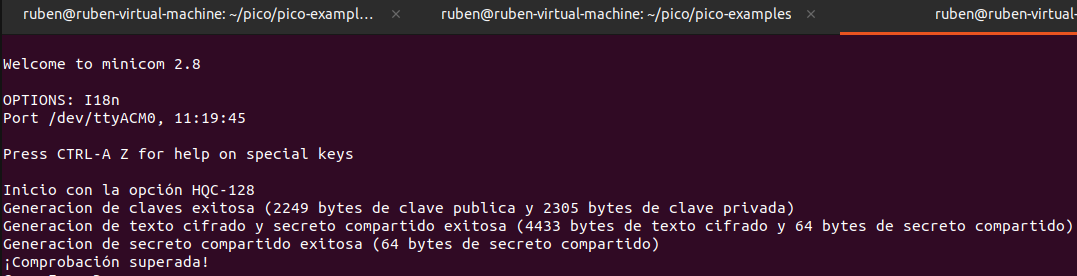
\includegraphics[width=0.5\textwidth]{figures/hqc-check.png}
    \caption{Comprobación de ejecución de algoritmo HQC-128.}
    \label{fig:hqc-check}
\end{figure}


\subsection{McEliece348864}\label{subsec:mceliece}

Para este algoritmo, la implementación también se ha obtenido del repositorio del proyecto PQClean~\cite{pqclean-github}.
En este caso, se ha contruido el árbol de ficheros mostrado en la Figura~\ref{tree:mceliece}.
Al igual que en los casos anteriores, se incluye un directorio \texttt{src} con los ficheros de código fuente y un directorio \texttt{include} en el que se incluyen todas las librerías del algoritmo.
Además, se incluye un archivo CMakeLists.txt y el fichero de comprobación \texttt{main.c}.

\begin{figure}[H]
\centering
\framebox[\textwidth]{%
\begin{minipage}{10cm}
\dirtree{%
.1 McEliece348864.
.2 main.c.
.2 CMakeLists.txt.
.2 src.
.3 aes256ctr.c.
.3 benes.c.
.3 bm.c.
.3 controlbits.c.
.3 crypto\_int16.c.
.3 crypto\_int32.c.
.3 crypto\_uint16.c.
.3 crypto\_uint32.c.
.3 crypto\_uint64.c.
.3 decrypt.c.
.3 encrypt.c.
.3 fips202.c.
.3 gf.c.
.3 operations.c.
.3 pk\_gen.c.
.3 randombytes.c.
.3 root.c.
.3 sk\_gen.c.
.3 synd.c.
.3 transpose.c.
.3 util.c.
.2 include.
.3 aes.h.
.3 aes256ctr.h.
.3 api.h.
.3 benes.h.
.3 bm.h.
.3 controlbits.h.
.3 crypto\_int16.h.
.3 crypto\_int32.h.
.3 crypto\_uint16.h.
.3 crypto\_uint32.h.
.3 crypto\_uint64.h.
.3 decrypt.h.
.3 encrypt.h.
.3 fips202.h.
.3 gf.h.
.3 main.h.
.3 operations.h.
.3 params.h.
.3 pk\_gen.h.
.3 randombytes.h.
.3 root.h.
.3 sk\_gen.h.
.3 synd.h.
.3 transpose.h.
.3 util.h.
}
\end{minipage}
}
\caption{Árbol de ficheros del proyecto MCEliece348864.}
\label{tree:mceliece}
\end{figure}


\subsubsection{Generación de números aleatorios}\label{subsubsec:mceliece-random}

Para adaptar la generación de números aleatorios en este algoritmo, se ha modificado el archivo \texttt{McEliece348864/src/rndombytes.c} de la forma mostrada en el Código~\ref{lst:mceliece-random}.
La función \texttt{randombytes} se utiliza para llamar a una función específica de generación de números aleatorios de acuerdo al sistema en el que se ejecuta, como por ejemplo Windows o un sistema basado en Linux.
Por ello, se debe crear una opción para el caso de RP2040, que se ha llamado \texttt{randombytes\_rp2040\_randombytes}.
El contenido de la función \texttt{randombytes\_rp2040\_randombytes} es idéntico a la función de generación de números aleatorios en el algoritmo HQC-128~\ref{subsubsec:hqc-random}.

\begin{lstlisting}[label={lst:mceliece-random},style=Cnice,firstnumber=1,caption={Archivo \texttt{McEliece348864/src/rndombytes.c}.}]
int randombytes(uint8_t *output, size_t n) {
    void *buf = (void *)output;
    #if defined(__EMSCRIPTEN__)
    ...
    #elif defined(RP2040)
    return randombytes_rp2040_randombytes(buf, n);
    #else
# error "randombytes(...) is not supported on this platform"
    #endif
}

#ifdef RP2040
static int randombytes_rp2040_randombytes(unsigned char *x, unsigned long long xlen){
    // srand(time(NULL));
    uint32_t aux = 0;
    for (int i = 0; i < xlen; i+=4){
        aux = get_rand_32();
        memcpy(x+i, &aux, min(4, xlen-1));
    }
    return 0;
}
#endif
\end{lstlisting}


\subsubsection{Fichero CMake}\label{subsubsec:mceliece-cmake}

En cuanto al fichero CMakeLists.txt, este contiene el Código~\ref{lst:mceliece-make}.
En él, se especifica el valor de la macro \texttt{PQCLEAN\_NAMESPACE} apropiado para la ejecución de este algoritmo junto al resto de opciones de compilación para mostrar los \textit{warning} existentes.
También, se incluyen todos los archivos fuente mostrados en el árbol~\ref{tree:mceliece}.
Además, se incluyen las dependencias comunes \texttt{stdlib} y \texttt{pico\_srand}.
Finalmente, se desactiva el uso de \ac{UART} como salida y se activa el uso de \ac{USB}.

\begin{lstlisting}[label={lst:mceliece-make},style=Cnice,firstnumber=1,caption={Archivo \texttt{McEliece348864/CMakeLists.txt}.}]
cmake_minimum_required(VERSION 3.13)

if (TARGET tinyusb_device)
    add_compile_options(-Wall -Wextra -Wpedantic -Wredundant-decls -Wcast-align -Wmissing-prototypes -DPQCLEAN_NAMESPACE=PQCLEAN_MCELIECE348864_CLEAN)

    add_executable(mceliece348864)

    target_sources(mceliece348864 PUBLIC
            ${CMAKE_CURRENT_LIST_DIR}/main.c
            ${CMAKE_CURRENT_LIST_DIR}/src/aes256ctr.c
            ${CMAKE_CURRENT_LIST_DIR}/src/benes.c
            ${CMAKE_CURRENT_LIST_DIR}/src/bm.c
            ${CMAKE_CURRENT_LIST_DIR}/src/controlbits.c
            ${CMAKE_CURRENT_LIST_DIR}/src/crypto_int16.c
            ${CMAKE_CURRENT_LIST_DIR}/src/crypto_int32.c
            ${CMAKE_CURRENT_LIST_DIR}/src/crypto_uint16.c
            ${CMAKE_CURRENT_LIST_DIR}/src/crypto_uint32.c
            ${CMAKE_CURRENT_LIST_DIR}/src/crypto_uint64.c
            ${CMAKE_CURRENT_LIST_DIR}/src/decrypt.c
            ${CMAKE_CURRENT_LIST_DIR}/src/encrypt.c
            ${CMAKE_CURRENT_LIST_DIR}/src/gf.c
            ${CMAKE_CURRENT_LIST_DIR}/src/operations.c
            ${CMAKE_CURRENT_LIST_DIR}/src/pk_gen.c
            ${CMAKE_CURRENT_LIST_DIR}/src/root.c
            ${CMAKE_CURRENT_LIST_DIR}/src/sk_gen.c
            ${CMAKE_CURRENT_LIST_DIR}/src/synd.c
            ${CMAKE_CURRENT_LIST_DIR}/src/transpose.c
            ${CMAKE_CURRENT_LIST_DIR}/src/util.c
            ${CMAKE_CURRENT_LIST_DIR}/src/randombytes.c
            ${CMAKE_CURRENT_LIST_DIR}/src/fips202.c
            )
    
    target_include_directories(mceliece348864 PUBLIC
                    ${CMAKE_CURRENT_LIST_DIR}/include)

    # pull in common dependencies
    target_link_libraries(mceliece348864 pico_stdlib pico_rand)

    # enable usb output, disable uart output
    pico_enable_stdio_usb(mceliece348864 1)
    pico_enable_stdio_uart(mceliece348864 0)

    # create map/bin/hex/uf2 file etc.
    pico_add_extra_outputs(mceliece348864)

    # add url via pico_set_program_url
    example_auto_set_url(mceliece348864)
elseif(PICO_ON_DEVICE)
    message(WARNING "not building mceliece348864 because TinyUSB submodule is not initialized in the SDK")
endif()
\end{lstlisting}


\subsubsection{Fichero de comprobación}\label{subsubsec:mceliece-main}

Para la comprobación del algoritmo, se ha utilizado el mismo archivo descrito en el apartado~\ref{subsubsec:hqc-main} ya que ambos incluyen funciones con el mismo nombre.
Únicamente se diferencian en el tamaño de las variables, lo cual viene indicado por la macro \texttt{PQCLEAN\_NAMESPACE} especcificada en el archivo CMakeLists.txt.
Además, las variables de claves pública y privada hacen uso de memoria dinámica en vez de memoria estática.


\subsubsection{Comprobación del algoritmo}\label{subsubsec:mceliece-comp}

Una vez completados estos pasos, se ha ejecutado el algoritmo utilizando el fichero descrito en el apartado~\ref{subsubsec:mceliece}.
El resultado de esta comprobación ha sido el mostrado en la Figura~\ref{fig:mceliece-check}.

\begin{figure}[h]
    \centering
    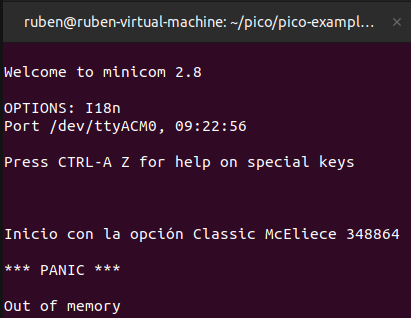
\includegraphics[width=0.5\textwidth]{figures/mceliece-check.png}
    \caption{Comprobación de ejecución de algoritmo McEliece348864.}
    \label{fig:mceliece-check}
\end{figure}

Como se puede verificar en la Figura~\ref{fig:mceliece-check}, la ejecución de este algoritmo arroja un error de memoria insuficiente.
Este error se genera al reservar memoria para las variables de las claves pública y privada.


\subsection{Sphincs}\label{subsec:sphincs}

El último algoritmo comprobado en este dispositivo se trata de Sphincs.
Para ello, se ha utilizado la implemantación oficial obtenible en el repositorio de GitHub~\cite{sphincs-github}.
En este repositorio, se encuentran varias implementaciones, entre las cuales se pueden ver una implementación optimizada para la arquitectura Intel x86 y de referencia en lenguaje C.
Para este trabajo, se ha utilizado la implementación de referencia incluida en el directorio \texttt{ref} del repositorio.
Para poder utilizar estos archivos, se ha creado el árbol de ficheros mostrado en la Figura~\ref{tree:sphincs}.
Al igual que con el resto de proyectos, todos los archivos fuente del algoritmo se han incluido en un directorio \texttt{src} mientras que las librerías se han  almacenado en el directorio \texttt{include}.

\begin{figure}[H]
\centering
\framebox[\textwidth]{%
\begin{minipage}{10cm}
\dirtree{%
.1 Spincs.
.2 main.c.
.2 CMakeLists.txt.
.2 src.
.3 address.c.
.3 fors.c.
.3 haraka.c.
.3 hash\_haraka.c.
.3 merkle.c.
.3 randombytes.c.
.3 sha2.c.
.3 sign.c.
.3 thash\_haraka\_robust.c.
.3 utils.c.
.3 utilsx1.c.
.3 wots.c.
.3 wotsx1.c.
.2 include.
.3 address.h.
.3 api.h.
.3 context.h.
.3 fors.h.
.3 haraka.h.
.3 haraka\_offsets.h.
.3 hash.h.
.3 merkle.h.
.3 params.h.
.3 randombytes.h.
.3 thash.h.
.3 utils.h.
.3 utilsx1.h.
.3 wots.h.
.3 wotsx1.h.
.3 params.
.4 params-sphincs-haraka-128f.h.
}
\end{minipage}
}
\caption{Árbol de ficheros del proyecto Sphincs.}
\label{tree:sphincs}
\end{figure}


\subsubsection{Fichero CMake}\label{subsubsec:sphincs-cmake}

En cuanto al fichero CMakeLists.txt, este contiene el Código~\ref{lst:sphincs-make}.
En él, se especifica el valor de la macro \texttt{PARAMS} apropiado para la ejecución de este algoritmo junto al resto de opciones de compilación para mostrar los \textit{warning} existentes.
También, se incluyen todos los archivos fuente mostrados en el árbol~\ref{tree:sphincs}.
Además, se incluyen las dependencias comunes \texttt{stdlib} y \texttt{pico\_srand}.
Por último, se activa el uso de \ac{USB} y se desactiva el uso de \ac{UART} como salida.

\begin{lstlisting}[label={lst:sphincs-make},style=Cnice,firstnumber=1,caption={Archivo \texttt{Sphincs/CMakeLists.txt}.}]
cmake_minimum_required(VERSION 3.13)

if (TARGET tinyusb_device)    
    add_compile_options(-Wall -Wextra -Wpedantic -Wconversion -Wmissing-prototypes -DPARAMS=sphincs-haraka-128f)

    add_executable(sphincs)

    target_sources(sphincs PUBLIC
            ${CMAKE_CURRENT_LIST_DIR}/main.c
            ${CMAKE_CURRENT_LIST_DIR}/src/address.c
            ${CMAKE_CURRENT_LIST_DIR}/src/randombytes.c
            ${CMAKE_CURRENT_LIST_DIR}/src/merkle.c
            ${CMAKE_CURRENT_LIST_DIR}/src/wots.c
            ${CMAKE_CURRENT_LIST_DIR}/src/wotsx1.c
            ${CMAKE_CURRENT_LIST_DIR}/src/utils.c
            ${CMAKE_CURRENT_LIST_DIR}/src/utilsx1.c
            ${CMAKE_CURRENT_LIST_DIR}/src/fors.c
            ${CMAKE_CURRENT_LIST_DIR}/src/sign.c
            ${CMAKE_CURRENT_LIST_DIR}/src/haraka.c
            ${CMAKE_CURRENT_LIST_DIR}/src/hash_haraka.c
            ${CMAKE_CURRENT_LIST_DIR}/src/thash_haraka_robust.c
            )
    
    target_include_directories(sphincs PUBLIC
                    ${CMAKE_CURRENT_LIST_DIR}/include
                    ${CMAKE_CURRENT_LIST_DIR}/include/params)

    # pull in common dependencies
    target_link_libraries(sphincs pico_stdlib pico_rand)

    # enable usb output, disable uart output
    pico_enable_stdio_usb(sphincs 1)
    pico_enable_stdio_uart(sphincs 0)

    # create map/bin/hex/uf2 file etc.
    pico_add_extra_outputs(sphincs)

    # add url via pico_set_program_url
    example_auto_set_url(sphincs)
elseif(PICO_ON_DEVICE)
    message(WARNING "not building sphincs because TinyUSB submodule is not initialized in the SDK")
endif()
\end{lstlisting}

En este proyecto, para modificar la versión del algoritmo utilizada, se debe modificar el archivo \texttt{Sphincs/CMakeLists.txt}.
Más concretamente, se debe cambiar el parámetro \texttt{PARAMS} de forma que especifique la función \textit{hash} utilizada (haraka o sha2), el número de bits a emplear (128, 192 o 256) y las opciones (s o f).
También, se puede elegir entre el archivo \texttt{/src/thash\_(función hash)\_robust.c} o \texttt{/src/thash\_(función hash)\_simple.c}.
En caso de seleccionar una función \textit{hash} distinta a haraka, se deben alterar las inclusiones \texttt{/src/haraka.c}, \texttt{/src/haraka.c} y \texttt{src/hash\_haraka.c}.
Para utilizar la función sha2, se debe sustituir ``haraka'' por ``sha2'' en el nombre de dichos archivos.
Para el caso de la función shake, se debe sustituir ``haraka'' por ``shake'' en el nombre de dichos archivos excepto \texttt{/src/haraka.c}, el cual se debe cambiar por \texttt{/src/fips202.c}


\subsubsection{Generación de números aleatorios}\label{subsubsec:sphincs-random}

Para la generación de números aleatorios, se ha utilizado el archivo \texttt{randombytes.c}, sustituyendo al inicialmente empleado \texttt{rng.c} ya que este se basaba en realizar operaciones a nivel de bit.
Por ello, se ha modificado la función que incluye el fichero \texttt{randombytes.c} para realizar la generación de números aleatorios mediante la función específica del dispositivo, ya que, originalmente, el archivo llevaba a cabo la generación mediante la apertura del fichero \texttt{/dev/urandom}, existente en los sistemas UNIX.
El contenido final de este fichero es el mostrado en el Código~\ref{lst:sphincs-random}.
Como se puede comprobar, la función \texttt{randombytes} es idéntica a las utilizadas en los algoritmos anteriores.

\begin{lstlisting}[label={lst:sphincs-random},style=Cnice,firstnumber=1,caption={Archivo \texttt{Sphincs/src/randombytes.c}.}]
#include <fcntl.h>
#include <unistd.h>
#include <string.h>
#include "pico/rand.h"
#include "randombytes.h"

void randombytes(unsigned char *x, unsigned long long xlen){
    uint32_t aux = 0;
    for (int i = 0; i < xlen; i+=4){
        aux = get_rand_32();
        memcpy(x+i, &aux, min(4, xlen-1));
    }
}
\end{lstlisting}

\subsubsection{Fichero de comprobación}\label{subsubsec:sphincs-main}

Para poder comprobar el algoritmo Sphincs, se ha diseñado el archivo \texttt{main.c} con el contenido mostrado en el código~\ref{lst:sphincs-main}.
En este fichero se ha seguido la nomenclatura seguida hasta, por lo que las claves pública (\texttt{pk}) y privada (\texttt{sk}) mediante la función \texttt{crypto\_sign\_keypair}.
A continuación, se utiliza la clave pública para firmar un mensaje (\texttt{m} con longitud \texttt{mlen}) utilizando la función \texttt{crypto\_sign}, la cual nos devuelve el mensaje firmado \texttt{sm} con longitud \texttt{smlen}.
Por último, se obtiene el mensaje firmado (\texttt{m1} con longitud \texttt{mlen1}) con la función \texttt{crypto\_sign\_open} y se verifica si es idéntico al firmado originalmente.

\begin{lstlisting}[label={lst:sphincs-main},style=Cnice,firstnumber=1,caption={Archivo \texttt{Sphincs/main.c}.}]
#include <stdio.h>
#include <stdlib.h>
#include <string.h>
#include "pico/stdlib.h"
#include "api.h"

int main() {
    stdio_init_all();
    printf("Inicio con la opción %s\n\r", xstr(PARAMS));

    //Generación de claves
    unsigned char pk[CRYPTO_PUBLICKEYBYTES], sk[CRYPTO_SECRETKEYBYTES];

    //Firma de mensaje
    unsigned char m[] = "Esto es una prueba de la firma de mensajes utilizando Sphincs.";
    unsigned char *sm;
    unsigned long long mlen = sizeof(m), smlen;

    //Comprobación de la firma
    unsigned char *m1;
    unsigned long long mlen1;

    while (true) {
        //Generación de claves
        printf("Inicio\n");
        if (crypto_sign_keypair(pk, sk)!= 0){
            printf("Generacion de claves fallida\n\r");
        } else {
            printf("Generacion de claves exitosa (%d bytes de clave publica y %d bytes de clave privada)\n\r", CRYPTO_PUBLICKEYBYTES, CRYPTO_SECRETKEYBYTES);
        }

        //Firma de mensaje
        m1 = (unsigned char *)calloc(mlen+CRYPTO_BYTES, sizeof(unsigned char));
        sm = (unsigned char *)calloc(mlen+CRYPTO_BYTES, sizeof(unsigned char));
        if (crypto_sign(sm, &smlen, m, mlen, sk) != 0){
            printf("Firma de mensaje fallida\n\r");
        } else {
            printf("Firma del mensaje exitosa (%llu bytes de firma)\n\r", smlen);
        }

        //Comprobación de la firma
        if (crypto_sign_open(m1, &mlen1, sm, smlen, pk) != 0) {
            printf("Comprobacion de la firma fallida\n\r");
        } else {
            if (mlen != mlen1) {
                printf("Longitud del mensaje original distinta a la longitud del mensaje recuperado\n\r");
            } else if (memcmp(m, m1, mlen)) {
                printf("Contenido del mensaje original distinto al contenido del mensaje recuperado\n\r");
            } else {
                printf("Comprobacion de la firma del mensaje exitosa (%llu bytes de mensaje)\n\r", mlen1);
            }
        }

        //Liberación de la memoria reservada
        free(m1);
        free(sm);
        sleep_ms(10000);
    }
}
\end{lstlisting}


\subsubsection{Comprobación del algoritmo}\label{subsubsec:sphincs-comp}

Finalmente, se ha llevado a cabo la ejecución del fichero de comprobación y se ha obtenido el resultado mostrado en la Captura~\ref{fig:sphincs-check}.

\begin{figure}[h]
    \centering
    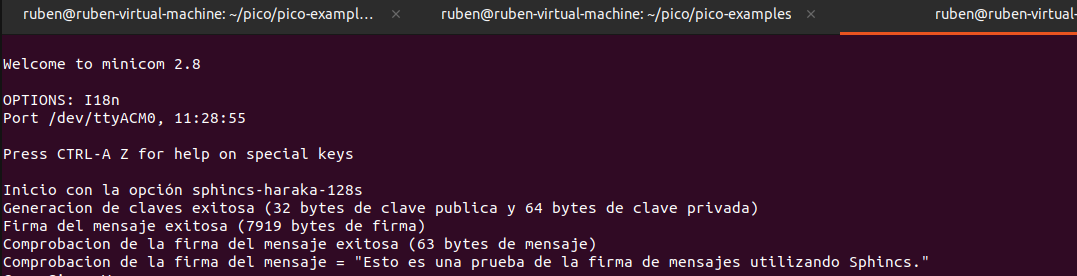
\includegraphics[width=0.5\textwidth]{figures/sphincs-check.png}
    \caption{Comprobación de ejecución de algoritmo Sphincs.}
    \label{fig:sphincs-check}
\end{figure}



\section{STM32}\label{sec:stm32}

El último dispositivo a utilizar se trata del dispositivo STM32, específicamente de la plataforma Nucleo-L4R5ZI.

Para poder programar esta plataforma, se disponen de dos posibilidades principales: Keil $\mu$Vision5~\cite{keil} y STM32Cube~\cite{stm32cube}.
STM32Cube se trata de una herramienta oficial desarrollada por el grupo ST.
Esta herramienta incluye los módulos:

\begin{itemize}
    \item \textbf{STM32CubeMX}~\cite{stm32cubemx}: Es un módulo gráfico utilizado para cualquier dispositivo STM32 el cual genera el código de inicialización en lenguaje C.
    \item \textbf{STM32CubeIDE}~\cite{stm32cubeide}: Este \ac{IDE} se basa en soluciones como Eclipse y aporta un compilador y depurador.
    \item \textbf{STM32CubeMonitor}~\cite{stm32cubemonitor}: Este módulo provee la posibilidad de comprobar datos de la aplicación en tiempo real.
    \item \textbf{STM32CubeProgrammer}~\cite{stm32cubeprogrammer}: Este módulo proporciona una manera de leer y escribir en la memoria del dispositivo en tiempo real.
\end{itemize}

Como inconveniente, esta herramienta requiere un tiempo excesivo para su dominio ya que entraña gran complejidad.
Por el contrario, Keil $\mu$Vision5 supone una menor dificultad por lo que será la herramienta utilizada.


\subsection{Keil uVision5}\label{subsec:keil}

Este \textit{software} hace uso de librerías, módulos y ficheros de configuración específicos de los dispositivos utilizados.
Para ello, se debe seleccionar el dispositivo utilizado en el menú ofrecido por la herramienta.

Para poder cargar \textit{software} en el dispositivo, es necesario llevar a cabo la especificación del rango de memoria disponible para la carga del programa.
Esto se realiza mediante la ventana a \texttt{Cortex-M Target Driver Setup}, a la cual se puede acceder desde la configuración del proyecto y, dentro de ella, el apartado ``Settings'' dentro de la ventana ``Utilities''.
Dentro de esta ventana, se debe seleccionar la opción ``Add'' y añadir la opcion con nombre ``STM32L4Rx 2MB Dual Bank Flash'', con dirección de inicio 0x800\_0000 y tamaño 0x20\_0000.
También, se debe indicar la RAM disponible para el algoritmo.
Esta comienza en la dirección de memoria 0x2000\_0000 y con un tamaño 0xA\_0000.

\subsection{McEliece348864}\label{subsec:mceliece-stm}

Para la ejecución del algoritmo McEliece348864, en primer lugar, se requiere la selección del código fuente.
Dicho código fuente se obtiene del repositorio perteneciente al proyecto PQClean~\cite{pqclean-github}.

Una vez se disponga del código, este se incluye en el projecto de ejemplo que se menciona en la Subsección~\ref{subsubsec:stm32-random}.


\subsubsection{Generación de números aleatorios}\label{subsubsec:stm32-random}

Para la generación de números aleatorios, se ha utilizado el ejemplo propuesto en el repositorio STM32CubeL4~\cite{stm32cubeL4}.
Este ejemplo se encuentra en la ruta \texttt{STM32CubeL4/Projects/NUCLEO-L4R5ZI/Examples/RNG/RNG\_MultiRNG}.
En este ejemplo, se utiliza la función \texttt{HAL\_RNG\_GenerateRandomNumber}, la cual obtiene números aleatorios de 32 bits.
Por ello, se ha diseñado la función \texttt{randombytes\_stm32\_randombytes} para su uso en el algoritmo.
Esta función se muestra en el Código~\ref{lst:mceliece-random}.

\begin{lstlisting}[label={lst:mceliece-random},style=Cnice,firstnumber=1,caption={Función de generación de números aleatorios para McEliece348864.}]
int randombytes_stm32_randombytes(unsigned char *x, unsigned long long xlen){
    // srand(time(NULL));
    uint32_t aux = 0;
    for (int i = 0; i < (int) xlen; i+=4){
        HAL_RNG_GenerateRandomNumber(&RngHandle, &aux);
        memcpy(x+i, &aux, min(4, xlen-1));
    }
    return 0;
}
\end{lstlisting}

\subsubsection{Archivo \texttt{startup\_stm32l4r5xx.s}}\label{subsubsec:mceliece-startup}

A continuación, se debe llevar a cabo la modificación del archivo \texttt{startup\_stm32l4r5xx.s}.
En este archivo se indica el puntero a la pila y el manejador de la interrupción de reinicio entre otras opciones al iniciar el dispositivo.
Además, se indica le tamaño de la memoria \textit{stack}, que inicialmente es 0x400.
Este valor provoca que la ejecución del programa arroje un error a la hora de llamar a la función \texttt{pk\_gen} en el archivo \texttt{pk\_gen.c}.
Los errores arrojados se muestran en la Figura~\ref{fig:mceliece-error}.
Ambos errores se refieren a un uso erróneo de la memoria \textit{stack}.

\begin{figure}[h]
    \centering
    \begin{subfigure}[b]{0.3\textwidth}
        \centering
        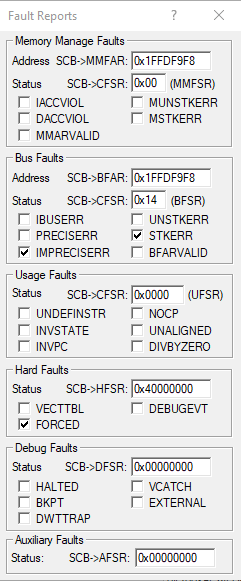
\includegraphics[width=\textwidth]{figures/keil_error_5A000.png}
        %\caption{Tiempos de convergencia en nRF52840 DK sin utilizar \textit{logs}.}
        %\label{subfig:nrf_sin_log}
    \end{subfigure}
    \hspace{1.5cm}
    \begin{subfigure}[b]{0.3\textwidth}
        \centering
        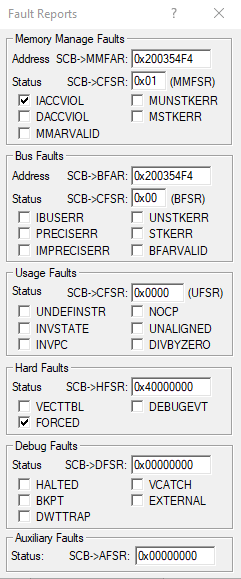
\includegraphics[width=\textwidth]{figures/keil_error_5B500.png}
        %\caption{Tiempos de convergencia en nRF52840 DK utilizando \textit{logs}.}
        %\label{subfig:nrf_con_log}
    \end{subfigure}
       \caption{Errores de manejo de memoria \textit{stack} al ejecutar McEliece348864.}
       \label{fig:mceliece-error}
\end{figure}

Dicho error se debe a que las variables utilizadas en dicha función no caben en la memoria \textit{stack}.
Las definiciones de las variables más grandes se muestran en el Código~\ref{lst:mceliece-pk-gen}.

\begin{lstlisting}[label={lst:mceliece-pk-gen},style=Cnice,firstnumber=1,caption={Variables en la función \texttt{pk\_gen}.}]
#define GFBITS 12
#define SYS_N 3488
#define SYS_T 64
#define PK_NROWS (SYS_T*GFBITS)

typedef uint16_t gf;

...

uint64_t buf[ 1 << GFBITS ];

unsigned char mat[ PK_NROWS ][ SYS_N / 8 ];

gf g[ SYS_T + 1 ]; // Goppa polynomial
gf L[ SYS_N ]; // support
gf inv[ SYS_N ];
\end{lstlisting}

La variable \texttt{buf} utiliza 32.768 bytes (0x800), lo cual ya es superior al tamaño de la memoria \textit{stack} asignada inicialmente.
La variable \texttt{mat} hace uso de 334.848 bytes (0x5\_1C00).
La variable \texttt{g} emplea 130 bytes (0x82) mientras que las variables \texttt{L} y \texttt{inv} requieren 6.976 bytes (0x1B40) cada una.
En total, el tamaño requerido de memoria \textit{stack} en esta función es de 381.650 bytes (0x5D2D2).
Por ello, se debe asignar un tamaño mínimo a la memoria \textit{stack} suficiente para llevar a cabo la ejecución del \textit{software} pero no tanta como para que no sea posible almacenar el código ejecutable, lo cual sucede al asignar 0x6\_0000 bytes a la memoria \textit{stack}.
La cantidad de memoria utilizada finalmente ha sido 0x5D800.


\subsubsection{Función de encapsulado y desencapsulado}\label{subsubsec:mceliece-dec-enc}

Como se ha indicado en la Subsección~\ref{subsubsec:mceliece-startup}, para la ejecución de la función \texttt{pk\_gen} se ha de aumentar el tamaño de la memoria \textit{stack} casi hasta el máximo posible.
Esto cubre únicamente la generación de claves del algoritmo.
Al incluir las funciones de encapsulado y desencapsulado se obtiene el mismo error que se recibía inicialmente para la función de generación de claves.
Esto hace que no sea viable la ejecución de la función de encapsulado y desencapsulado del algoritmo ya que no son manejables debido al tamaño disponible de memoria.


\subsection{PQM4}\label{subsec:pqm4}

Para la ejecución de ortos algoritmos, se ha utilizado el repositorio existente PQM4~\cite{pqm4}.
Este repositorio contiene implementaciones de distintos algoritmos postcuánticos diseñadas para su uso en dispositivos que empleen microcontroladores pertenecientes a la familia ARM Cortex-M4.
Dentro de este repositorio, se pueden encontrar \textit{scripts} en Python 3 que llevan a cabo diferentes medidas de la ejecución de los distintos algoritmos en el dispositivo.
Estas medidas son el tiempo necesario para su ejecución, la cantidad de memoria \textit{stack} utilizada y el tamaño del código.
Algunas de las plataformas soportadas son Nucleo-L4R5ZI, Nucleo-L476RG, CW308T-STM32F3 y MPS2-AN386.

Para poder utilizar este \textit{software}, se debe instalar el paquete \texttt{arm-none-eabi-gcc} y OpenOCD.
Además, se debe utilizar una versión de Python igual o superior a la versión 3.8.

Para la obtención de las medidas de, por ejemplo, el algoritmo Bikel1, se ha de ejecutar el comando mostrado en el Código~\ref{lst:pqm4}.

\begin{lstlisting}[label={lst:pqm4},style=Cnice,firstnumber=1,caption={Comando para la obtención de medidas utilizando PQM4.}]
python3 benchmarks.py bikel1 --platform nucleo-l4r5zi --uart /dev/ttyACM1
\end{lstlisting}

Este comando arrojará las medidas obtenidas en diferentes archivos (según medida obtenida y algoritmo comprobado) dentro del directorio llamado \texttt{benchmarks}.

Para este proyecto, se ha llevado a cabo las medidas de los algoritmos Falcon (versiones 512 y 1024), Dilithium (versiones 2, 3 y 5), Kyber (versiones 2, 3 y 4), HQC (versiones 128, 192 y 256) y Bikel (versiones 1 y 3).


%%% Local Variables:
%%% TeX-master: "../book"
%%% End:
